\documentclass[12pt,a4paper]{article}

\usepackage[T2A]{fontenc}
\usepackage[utf8]{inputenc}

\usepackage[backend=biber]{biblatex}
\addbibresource{ref.bib}

\usepackage{amsmath}
\usepackage{commath}
\usepackage{titlesec}
\usepackage{graphicx}
\usepackage{caption}
\usepackage{indentfirst}
\usepackage{hyperref}
\usepackage{enumitem}[leftmargin=0pt]
\usepackage{multicol}
\usepackage{yfonts}
\usepackage{verbatim}
\usepackage{bm}
\usepackage{float}

\renewcommand{\vec}[1]{\bm{\mathrm{#1}}}


\begin{document}

\title{Precession of the Orbit of the Moon}
\author{Aleksandar Ivanov}
\date{\today}
\maketitle

\begin{abstract}
I study the effect of the Sun's gravity on the orbit of the moon by numerically simulating the Sun-Earth-Moon system within appropriate approximations. I find that two types of precession appear. Nodal, where the normal to the plane of the Earth-Moon orbit rotates around the normal of the Sun-Earth orbit, making the crossing points (nodes) rotate around with a period of $T_{nodal} \approx 18.5 \, \mathrm{years}$. And apsidal, where the major axis of the Moon's orbit rotates around the normal of the Earth-Moon orbit, making the apoapsis rotate with a period of $T_{apsidal} \approx 8.6 \, \mathrm{years}$.
\end{abstract}


\section{Background}

The Sun-Earth-Moon system is an example of a three-body gravitational problem. This kind of problem has been an interesting topic of Newtonian gravity ever since the discovery of the universal law of gravitation. It is a complex enough problem that an analytic closed form solution for a generic configuration is not possible. Progress can be made analytically only by looking at specific configurations with appropriate approximations. \cite{srbisols}

Another method to get to a solution of the problem is to use numerical simulation to iteratively solve the differential equations of motion. This method works relatively well for the three-body problem but quickly gets complicated as the number of masses $N$ is increased because each mass needs $6$ coordinates to describe its motion, which leaves us with a $6N$-dimensional phase space not counting constraints.

This suggests that we need to be smarter in utilizing numerical methods and that a combination of approximations and numerical simulations would be the easiest to work with, relative to the precision of the results that it provides.

The price that we have to pay for simplifying the problem in this way is that we need to make sure that the approximations are justified by the results. In other words, we have to do further work convincing ourselves that the results we are getting are not an artifact of the numerical analysis or the starting approximations.

\section{Setup of the problem}

The first obvious place to look for simplifications to the problem is in the masses. The masses of the bodies in the Sun-Earth-Moon system are \cite{podatoci}
%
\begin{align*}
\text{Sun: }& \mu = 1.988 \cdot 10^{30} \, \mathrm{kg} \\ 
\text{Earth: }& M = 5.972 \cdot 10^{24} \, \mathrm{kg} \\
\text{Moon: }& m = 7.346 \cdot 10^{22} \, \mathrm{kg}.
\end{align*}
%

It's clear that this lends itself nicely to approximations of the kind $\mu \gg M \gg m$. In particular $\mu \gg M, \, m $ leads us to say

\vspace{0.35cm}
\noindent
\textbf{Approx. 1:} Throughout the motion the Sun remains stationary.
\vspace{0.35cm}

\noindent
and, moreover $M \gg m $ leads us to say

\vspace{0.35cm}
\noindent
\textbf{Approx. 2:} The Earth's motion is determined solely by the Sun's gravity.
\vspace{0.35cm}

The next place to look for simplifications is in the shape of the Earth's orbit. Because of the second approximation, we know that the Earth's orbit will be an ellipse. But the orbital eccentricity in the case of the Earth is found to be $\mathcal{E} = 0.0167$. \cite{podatoci}

Plugging into the equation
%
\begin{align}
\mathcal{E}^2 = 1 - \frac{B^2}{A^2}
\end{align}
%
where $A$ is the semi-major axis and $B$ is the semi-minor axis, we get that the error in the distance we get by taking $A = B = R$ is only around $0.01 \%$, which justifies

\vspace{0.35cm}
\noindent
\textbf{Approx. 3:} The Earth's orbit is circular.
\vspace{0.35cm}

Taking these approximations into account, we can define a coordinate system such that the Sun is at the origin and the Sun-Earth orbit lies in the $x-y$ plane. In such a coordinate system, we describe the positions of the Earth and the Moon with the following coordinates:
%
\begin{align}\label{coords}
&\text{Earth} && \text{Moon}& \nonumber \\
X &= R \cos(\Omega t + \phi) && x = x(t)& \nonumber \\
Y &= R \sin(\Omega t + \phi) && y = y(t)& \nonumber \\
Z &= 0 && z = z(t)&
\end{align}
%
where $x(t)$, $y(t)$ and $z(t)$ are functions that will be determined by the differential equations, $R = 1.496 \cdot 10^{11} \, \mathrm{m}$ is the orbital radius of the Earth, $\Omega = 1.991 \cdot 10^{-7} \, \mathrm{s^{-1}}$ is the angular speed of the Earth's orbit and $\phi$ is a phase that will be determined by the initial conditions.

The equations of motion are given by simple application of Newton's II law and in component form they are:
%
\begin{align}
\ddot{x} &= - \frac{G \mu x}{\left[x^2 + y^2 + z^2\right]^{3/2}} - \frac{G M (x - X)}{\left[(x - X)^2 + (y - Y)^2 + z^2\right]^{3/2}} \\
%
\ddot{y} &= - \frac{G \mu y}{\left[x^2 + y^2 + z^2\right]^{3/2}} - \frac{G M (y - Y)}{\left[(x - X)^2 + (y - Y)^2 + z^2\right]^{3/2}} \\
%
\ddot{z} &= - \frac{G \mu z}{\left[x^2 + y^2 + z^2\right]^{3/2}} - \frac{G M z}{\left[(x - X)^2 + (y - Y)^2 + z^2\right]^{3/2}}
\end{align}
%
where $G = 6.674 \cdot 10^{-11} \, \mathrm{m^3 \, kg^{-1} \, s^{-2}}$ is the universal gravitational constant and $X$ and $Y$ are as defined in \eqref{coords}.

Another fact that we have to take into consideration is that the Earth-Moon orbit is inclined relative to the ecliptic by $\delta = 5.145 ^{\circ}$. \cite{podatoci} This inclination will be encoded in the initial conditions.

The periods of the orbits of the Moon around the Earth and the Earth around the Sun are not in a rational ratio of eachother which means that the system will eventually visit all possible configurations. This allows us to pick any configuration as our starting one. Specifically, we can pick one that makes the initial conditions the easiest to write down.

For the Earth, we will choose the initial condition
%
\begin{align}
\phi = 0
\end{align}
%
which places it on the $x$ axis with no $y$ or $z$ components of position.

For the Moon, we will choose the initial conditions
%
\begin{align}
x(0) &= R + a (1 + \epsilon) \cos \delta && \dot{x}(0) = 0& \nonumber \\
y(0) &= 0 && \dot{y}(0) = R \Omega + v_a& \nonumber \\
z(0) &= a (1 + \epsilon) \sin \delta && \dot{z}(0) = 0&
\end{align}
%
where $a = 3.844 \cdot 10^{8} \, \mathrm{m}$ is the semi-major axis of the Moon's orbit, $\epsilon = 0.0549$ is it's eccentricity and $v_a$ is the aphelion velocity of the Moon in the Earth-Moon system which can be calculated from approximate conservation of energy for that system and is found to be
%
\begin{align}
v_a = \sqrt{\frac{G M}{a} \, \frac{1 - \epsilon}{1 + \epsilon}} = 970 \, \mathrm{m \, s^{-1}}.
\end{align}

This configuration represents the Moon being at aphelion at $t = 0$ and the semi-major axis of the Moon lying in the $x-z$ plane.

Another thing to note is that $\mu$, $R$ and $\Omega$ are correlated and it's only necessary to know two of them. In practice the mass of the Sun $\mu$ is calculated from the other two as
%
\begin{align}
G \mu = \Omega^2 R^3,
\end{align}
%
so we will use $R$ and $\Omega$ as our parameters.

Our final list of parameters for our simulation is then given as \cite{podatoci}
%
\begin{multicols}{2}
\begin{enumerate}
\item $G = 6.674 \cdot 10^{-11} \, \mathrm{m^3 \, kg^{-1} \, s^{-2}}$

\item $M = 5.972 \cdot 10^{24} \, \mathrm{kg}$

\item $m = 7.346 \cdot 10^{22} \, \mathrm{kg}$

\item $R = 1.496 \cdot 10^{11} \, \mathrm{m}$

\item $\Omega = 1.991 \cdot 10^{-7} \, \mathrm{s^{-1}}$

\item $a = 3.844 \cdot 10^{8} \, \mathrm{m}$

\item $\epsilon = 0.0549$

\item $\delta = 5.145 ^{\circ}$
\end{enumerate}
\end{multicols}

\section{Methods}

The orbit of the Moon is observed to represent an ellipse relatively closely. That means that all the effects due to the Sun can be considered as perturbations to that elliptical orbit.

The Sun will provide an external torque acting on the rotating Moon. Any such system where a torque has a component perpendicular to the angular momentum of a body exibits precession of that angular momentum vector \cite{morinclassical}. We can expect that such an effect will be apparent in the simulation.

Thus, one of the things we want from the code is to track the components of the normalized angular momentum or normal vector to the orbit
%
\begin{align}\label{normal}
\vec{n} = \frac{\vec{L}}{\abs{\vec{L}}} = \frac{\vec{\rho} \times \vec{v}}{\abs{\vec{\rho} \times \vec{v}}}
\end{align}
%
from which we will then extract the period of nodal precession. The $\vec{\rho}$ in \eqref{normal} is the radial distance vector of the Moon from the Earth, and $\vec{v}$ is the velocity of the Moon with respect to the Earth.

The extraction of the period will be done by calculating the autocorrelation so as to surpress the noise coming from other effects and numerical errors, and then looking at neighbouring maxima and the difference of their corresponding times.

As shown in \textcite{apsidalcalc}, another effect that appears as a result of the Sun's perturbation is the precession of the major axis of the orbit of the Moon.

To see this effect manifestly, we will define an angle
%
\begin{align}
\theta = \arccos \left( \frac{\vec{\rho} \cdot \vec{\tilde{x}}}{\abs{\vec{\rho}} \abs{\vec{\tilde{x}}}} \right)
\end{align}
%
where
%
\begin{align}
\vec{\tilde{x}} = \vec{\hat{x}} - \left( \vec{n} \cdot \vec{\hat{x}} \right) \vec{n}
\end{align}
%
is the projection of the $x$-axis onto the plane of the orbit. This angle tells us the Moon's angular position in it's orbit around the Earth.

Then we need to find the apoapsides at different times by finding the maxima of $\abs{\vec{\rho}}$ and their corresponding angles $\theta_a$ and times $t_a$. By tracking for which $t_a$ the angles $\theta_a$ make a full rotation we get the period of apsidal precession.

\section{Results}

The precession of the plane of the orbit of the Moon  is most easily visualized by plotting the components of the normal vector as functions of time, as in Figure \ref{compsofn}. The figure clearly shows that the $x$ and $y$ components oscillate and, moreover, that they are out of phase by $\frac{\pi}{2}$, while the $z$ component comparatively doesn't change by much.

This exemplifies two facts. Firstly, because the $z$ component doesn't oscillate we know that the normal vector executes its rotation around the $z$-axis. And secondly, because the $x$ and $y$ components' oscillations have that exact form and phase shift of $\frac{\pi}{2}$, the vector's tip traces out a circle.

The period of those oscillations gives us the period of nodal precession as $T_{nodal} = 18.48 \, \mathrm{years}$. As expected, this is much bigger than a period of the orbit which justifies the assumption that the Sun's effect acts only as a perturbation to the originally elliptical orbit.

Measurements of the actual period of nodal precession are done by measuring when the ascending node makes a full rotation relative to the vernal equinox. The ascending node is defined as the point at which the Moon crosses the ecliptic upwards as viewed from our coordinate system. These give the value for the period as $T_{nodal}^{meas.} = 18.597 \, \mathrm{years}$. The relative error of the value we get compared to the actual value is around $0.63 \, \%$. We can see that the agreement between the simulation and the real system is really good, despite the approximations made.

\begin{figure}[H]
\centering
\captionsetup{justification = centering}
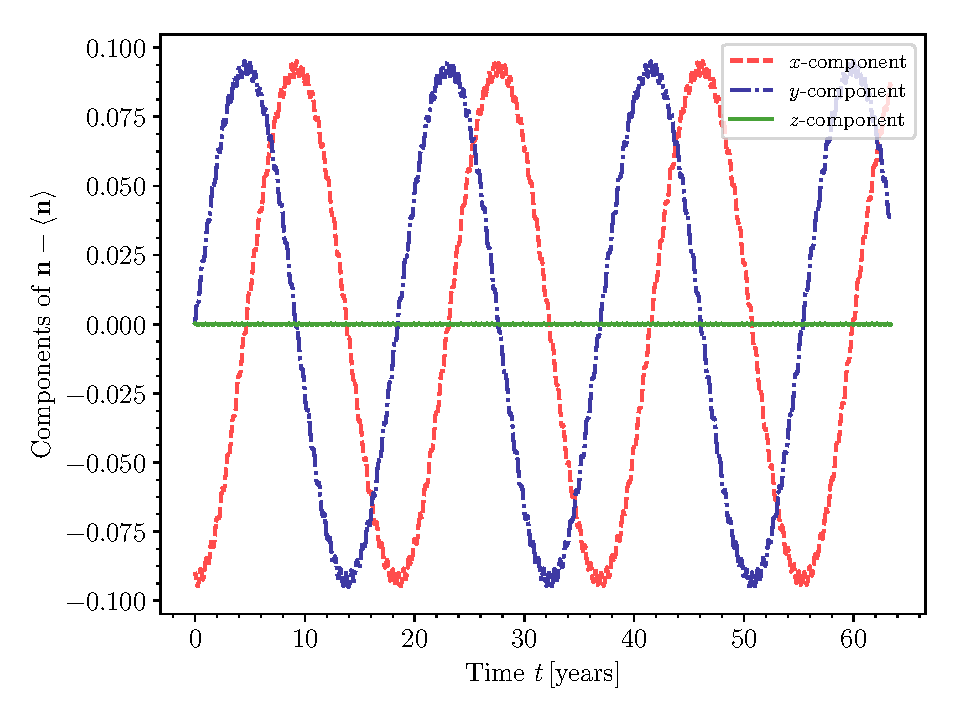
\includegraphics[scale = 0.8]{compsofn.pdf}
\caption{The oscillations of the components of the normal vector to the plane of the orbit about their averages. The $x$-component is shown in dashed red, the $y$-component in dotdashed blue and the $z$-component in full green. It can clearly be seen that the normal vector precesses around the $z$-axis.}
\label{compsofn}
\end{figure}

The result of the apsidal precession is that from apoapsis to apoapsis, the Moon goes through a bit more than $2 \pi$ radians. Numerically, the result will appear in the angles at which we reach apoapsis. Figure \ref{apotheta} shows these angles $\theta_a$ as a function of time $t_a$, but they're plotted modulo $2 \pi$ to accentuate their periodicity in the sense of the orbit.

Another useful convention for the angles $\theta_a$ is where we take them to be a growing, instead of a periodic, function of time. In this case we get an approximately linear graph as implied by Figure \ref{apotheta} which can be used to easily determine the period as
%
\begin{align}
T_{apsidal} = \frac{2 \pi}{\Delta \theta_a / \Delta t_a}
\end{align}
%
where $\Delta \theta_a / \Delta t_a$ is the slope of the linear graph of $\theta_a$ vs. $t_a$.

The period determined in this way is $T_{apsidal} = 8.55 \, \mathrm{years}$. Again, this result justifies the assumption of looking at the Sun's results as a perturbation because it is much bigger than a month.

Comparing to the actual measured value of $T_{apsidal}^{meas.} = 8.851 \, \mathrm{years}$ we get a relative error of $3.4 \, \%$ which is, again, in very good agreement with measurements.

\begin{figure}[H]
\centering
\captionsetup{justification=centering}
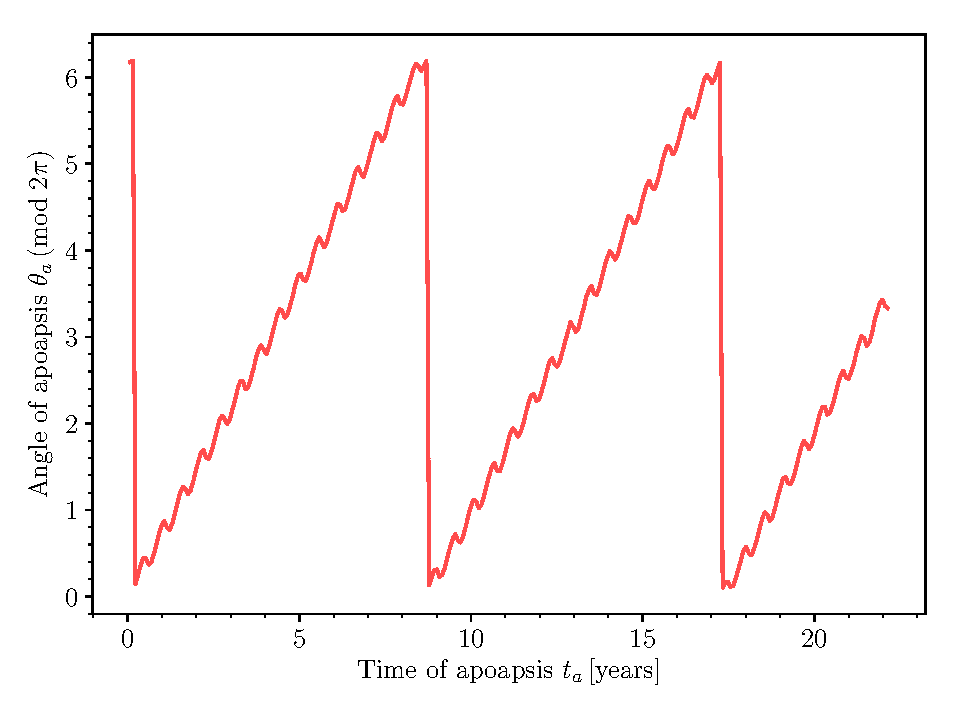
\includegraphics[scale = 0.8]{apothetavst.pdf}
\caption{The angles of apoapsis $\theta_a$ plotted against time $t_a$. The angles are plotted modulo $2 \pi$ to allude to the fact that the motion is still approximately periodic.}
\label{apotheta}
\end{figure}

\newpage

\printbibliography

\end{document}